\documentclass[conference, letterpaper, 10pt, times]{IEEEtran}

\usepackage[T1]{fontenc}
\usepackage{amsfonts}
\usepackage{amsmath}
\usepackage{bm}

\usepackage[dvipsnames]{xcolor}
\usepackage{graphicx}

\usepackage[binary-units, per-mode=symbol]{siunitx}
\sisetup{range-phrase=--, range-units=single}

\usepackage[basic]{complexity}
\usepackage[super,negative]{nth}

\usepackage{booktabs}
\usepackage{microtype}

%% Fix indent in new section...
\newcommand{\subparagraph}{}
\usepackage{titlesec}
\titlespacing*{\section}{0pt}{1.5ex}{0.7ex}
\titlespacing*{\subsection}{0pt}{1.5ex}{0.7ex}
%\titleformat*{\filcenter\scshape}

%bib
\usepackage[maxnames=3,maxbibnames=99,mincrossrefs=5,style=ieee,sortcites,backend=bibtex]{biblatex}
\addbibresource{papers-off.bib}
\addbibresource{confs-off.bib}
\addbibresource{books-off.bib}
\addbibresource{rfc.bib}
\addbibresource{misc.bib}

%picky abt et al.
\usepackage{xpatch}

\xpatchbibmacro{name:andothers}{%
	\bibstring{andothers}%
}{%
	\bibstring[\emph]{andothers}%
}{}{}
\DeclareFieldFormat[inproceedings]{url}{}
\DeclareFieldFormat[article]{url}{}

%opening!

\newcommand{\mytitle}{Improving Direct-Control Reinforcement Learning for Network Intrusion Prevention}

\usepackage{url}
\usepackage{hyperref}
\usepackage{cleveref}
\newcommand{\crefrangeconjunction}{--}

\hypersetup{
	colorlinks,
	citecolor=black,
	filecolor=black,
	linkcolor=black,
	urlcolor=black,
	pdftitle={\mytitle{}},
	pdfauthor={Kyle A. Simpson}
}
\newcommand*{\email}[1]{\href{mailto:#1}{\nolinkurl{#1}} } 

\usepackage{titling}
\settowidth{\thanksmarkwidth}{*}
\setlength{\thanksmargin}{-\thanksmarkwidth}

%% Enable /thanks
\IEEEoverridecommandlockouts
\makeatletter
\def\footnoterule{\relax%
	\kern-5pt
	\hbox to \columnwidth{\hfill\vrule width 0.5\columnwidth height 0.4pt\hfill}
	\kern4.6pt}
\makeatother

% make math easy
\newcommand{\acval}[3]{\ensuremath{\operatorname{\hat{q}}(#1, #2, #3)}}
\newcommand{\wvec}[1]{\ensuremath{\bm{w}_{#1}}}

%-------------------------------------%
%-------------------------------------%

\title{\mytitle{}}
\author{Kyle A. Simpson\thanks{This work was supported by the Engineering and Physical Sciences
		Research Council [grant number EP/M508056/1]}\\University of Glasgow, Glasgow, Scotland,\\
		\email{k.simpson.1@research.gla.ac.uk}}

% Remove date, leave no spacing.
\predate{}
\postdate{}
\date{}

\begin{document}

%% If needed, make urls typewritery
%\urlstyle{tt}

\maketitle

\begin{abstract}
Network intrusion detection and prevention systems backed by machine learning (and the autonomous operation they promise) have been long-heralded, but face problems hampering effective deployment.
The detection problem in this domain is fraught with difficulty; it is an evolving, non-stationary problem as usage patterns shift, new protocols and applications are introduced, compounded by burstiness and seasonal variation.

\emph{Reinforcement learning} (RL) may overcome the detection problem for certain classes of anomaly by managing and monitoring \emph{consequences}; an agent's role is to learn to optimise performance criteria (which are always available).

I present...
?? Contribs

?? Taking up space to figure out how much room I have for an intro

?? still taking up space...

?? still going...

?? done...
\end{abstract}

\section{Introduction}

Network anomaly detection, intrusion detection and intrusion prevention are continually evolving problems, compounded by the partial, non-IID view of data at each point in the network.
Attacks and anomalous behaviours evolve, becoming more sophisticated or employing new vectors to harm a network or system's confidentiality, integrity, or availability without being detected.
These attacks and anomalies have measurable consequences and symptoms which allow a skilled analyst to infer new signatures for detection by misuse-based classifiers, but unseen attacks may only be defended against after-the-fact.

While \emph{machine learning} (ML) approaches seem like a sensible fit for this problem, in \citeyear{DBLP:conf/sp/SommerP10} \textcite{DBLP:conf/sp/SommerP10} identified the `failure to launch' of ML-based anomaly detection systems---to quite a large extent, this remains the case today.
Their application is made difficult due to significant operational differences from standard ML tasks, alongside certain characteristics of network traffic.
Briefly, these are the diversity of network traffic across varying timescales \cite{DBLP:conf/sp/SommerP10} and significant burstiness \cite{DBLP:journals/ccr/LelandWTW95}.
Above the aggregate level, the constant deployment of new services and new protocols means that traffic is \emph{non-stationary} and displays an evolving notion of normality.
This is compounded by the extraordinarily low tolerance for false positives inherent to network intrusion detection \cite{DBLP:conf/ccs/Axelsson99}, and the challenges of learning from unlabelled (often partial) data.
All of these factors greatly inflate the difficulty of the detection problem.

For certain classes of problem like non-transit DDoS attacks, \emph{reinforcement learning} (RL) is best-posed to adaptively react to certain classes of threat by assuming the role of a feedback loop for network optimisation, typically to safeguard service guarantees.
In a sense, this allows us to ``overcome'' the difficulties of the detection problem by monitoring \emph{performance characteristics and consequences} in real-time, by looking for the effect rather than the cause.
The intent is to augment what existing solutions can provide, by automatically alerting, recording and controlling what are believed to be illegal system states.
%Whether it takes direct control of the network, or is used indirectly to optimise a key part of another system, more powerful `deep' RL techniques (and well-founded action spaces) aren't yet well explored for network IDS/IPS.
%These range from more modern training algorithms \cite{DBLP:journals/corr/SchulmanWDRK17, DBLP:conf/icml/SchulmanLAJM15}, to evolutionary strategies \cite{DBLP:journals/corr/SalimansHCS17, DBLP:journals/corr/abs-1802-08842}, hierarchical action composition \cite{DBLP:journals/corr/abs-1710-09767}, and competitive multi-agent learning \cite{DBLP:journals/corr/abs-1710-03748}.

?? Reference to the possible mistreatment of RL in our domain? The problem of ``blind application'' so hated by \textcite{DBLP:conf/sp/SommerP10}.

?? RL as a mechanism to protect systems by monitoring performance characteristics---overcome the detection problem (different handle on the key problems of burstiness, evolution, non-stationarity).

This paper contributes:
\begin{itemize}
	\item A DDoS mitigation system based on direct-control reinforcement learning designed for deployment in real-world software-defined networks.
	\item Important weaknesses and flaws in the past design and evaluation of similar techniques \cite{DBLP:journals/eaai/MalialisK15}---a deconstruction of their ISP-like formulation, and an acknowledgement of the flaws and risk factors of pushback \cite{DBLP:journals/ccr/MahajanBFIPS02a}.
	\item ?? TODO: Advance the use/representation/granularity of state-space in direct-control RL of networked applications.
\end{itemize}

\section{Background}

%?? Introduce RL, related definitions etc.
\emph{Reinforcement learning} (RL) is a variant of machine learning principally concerned with with training an agent to choose an optimal sequence of actions in the pursuit of a given task \cite{RL2E}.
We assume the agent has a certain amount of knowledge whenever a decision must be made: at any point in time $t$ it knows which \emph{state} it is in ($S_t \in \mathcal{S}$), the set of \emph{actions} which are available to it ($\mathcal{A} = A(S_t)$) and, if available, a numeric \emph{reward} obtained from the last action chosen ($R_t \in \mathbb{R}, A_t \in \mathcal{A}$).
RL methods combine this information with a current \emph{policy} $\pi$ to determine which action should be taken: such a choice need not be optimal, if an agent needs to further explore some region of the state space.
The policy is then further refined by updating value estimates for state-action pairs or via policy gradient methods, meaning that RL-based approaches learn adaptively and online if reward functions are available in their deployment environment.
From any point in a sequence of decisions, we may describe the sum of rewards yet to come as the \emph{return}, $G_t = R_{t+1} + \ldots + R_{t+T}$ for some (possibly infinite) choice of $T$.
Formally then, the goal is to maximise the \emph{expected return} $\operatorname{\mathbb{E}_{\pi}}[G_t | S_t]$ from any and all states $S_t$.

?? Include some details of function approximation in the formalisation? I.e. tile coding, stability and convergence guarantees...

There exists immense variation in \emph{how} policies and/or values may be learned, reliant upon the particular convergence guarantees required.

?? Is this \emph{actually} just sarsa? We're using fn approx (of course), but this is fraught with its own difficulties. Is it strictly speaking correct to describe it as Sarsa at this point? It's, at the very least, 1-step semi-gradient Sarsa given that it is clearly on-policy w/ fn approx...
?? IDEA: try out average reward, TD($\lambda$) methods as future work...

?? Discuss mininet? Networking terms? SDN stuff?

\section{A Plan, of Sorts}

\begin{enumerate}
	\item The main case for contribution in what I have so far:
	\begin{itemize}
		\item Past work reliant on unrealistic network models: tcp-like behaviour (and its effects on collateral damage) not captured, disjoint ranges of traffic distribution (no benign heavy-hitters), ISP-like topology.
		\item I offer more realistic network emulation environment, better treatment of protocol/traffic characteristics.
	\end{itemize}
	\item Forthcoming: rethinking state/action spaces to operate at a finer level of granularity. New network model (live tcp back-and-forth), allows us to test collateral damage assumptions in a more realistic manner (and show clear case for moving beyond work of malialis and kudenko)
\end{enumerate}

\section{Environment and RL Algorithm}

?? STRUCTURE: Either (methodology) -> (results) OR (their stuff + its weaknesses) -> (a new direction) [second is way punchier, but not yet ready to go with that.]

\subsection{Topology}
The network itself is tree-structured, where one server connects through a dedicated switch to $k$ team leader switches, each connected to $l$ intermediate switches, which in turn each connect to $m$ egress switches.
Agents are co-located with these egress switches, who control the proportion of upstream packets from $n$ external hosts to discard according to load statistics observed along their path to the server.
Agents communicate with their co-hosted OpenFlow-enabled switches---running a modified version of \emph{Open vSwitch} (OVS) \cite{open-vswitch}---to install probabilistic packet-drop rules.
Each link has a delay of \SI{10}{\milli\second}.
All links have unbounded capacity, save for the server-switch connection which is capped at a fixed $U_s$ \si{\mega\bit\per\second} in both directions.

?? Diagram? TikZ?

Reimplementation of the network model was performed using mininet \cite{mininet}, a Python-based network emulator.
Traffic is played back from hosts via Tcpreplay at a bandwidth assigned uniformly from a `good' or `bad' distribution, each using the same pcap file with source and destination IP addresses rewritten.
While unrealistic with respect to packet content, it was assumed that this would provide representative load and packet inter-arrival characteristics, since the agents as initially defined are blind to such information.

\subsection{Agent Definitions}

?? Specify update rules here? Semi-gradient Sarsa \cite[pp.\ \numrange{243}{244}]{RL2E}? enhanced by tile-coding with identical parameter choices \cite{DBLP:phd/ethos/Malialis14}.

\begin{subequations}
\begin{align}
\delta_t = R_{t+1} + \gamma \acval{S_{t+1}}{A_{t+1}}{\wvec{t}} - \acval{S_t}{A_t}{\wvec{t}},\\
\bm{w}_{t+1} = \bm{w}_{t} + \alpha \delta_t \nabla{\acval{S_t}{A_t}{\wvec{t}}},
\end{align}
\end{subequations}
observing that the gradient is the binary vector of tile activations.

The reward functions as I specify them here were introduced by \textcite{DBLP:journals/eaai/MalialisK15}; in particular, I make use of the global reward as a performance metric and the \emph{coordinated team learning} (CTL) reward for training.
Using the Iverson bracket notation:
\begin{subequations}
\begin{align}
c_t^{\mathit{f}} = [ > U_s],\\
c_t^{\mathit{tf}} = [ > U_s/k],\\
R_{t}^{\mathit{Global}} = (1 - c_t^{\mathit{f}})\frac{a}{b} - c_t^{\mathit{f}},\\
R_{t}^{\mathit{CTL}} = (1 - c_t^{\mathit{f}}c_t^{\mathit{tf}})\frac{a}{b} - c_t^{\mathit{f}}c_t^{\mathit{tf}},
\end{align}
\end{subequations}

?? Note, these are dependent on the current agent! Need to find a succinct way to express this somehow...

?? M\&K Seem not to have a grasp on the importance of up/down traffic splits. Hmm......... (i.e., both could be relevant?)

?? wrt reward function relying on heuristic elements or perfect knowledge:
A sufficiently well-trained agent needs only to follow the policy it has learned in a greedy manner, allowing pre-training using a priori knowledge by simulation to transfer to reality.

\section{Performance in an Emulated Environment}

?? System specs of execution environment: 4-core Intel Core i7-6700K clocked at \SI{4.2}{\giga\hertz}, with \SI{32}{\gibi\byte} of RAM. All code is available on a public Github repository\footnote{\url{https://github.com/FelixMcFelix/rln-dc-ddos-paper}}.

\begin{figure}[ht]
	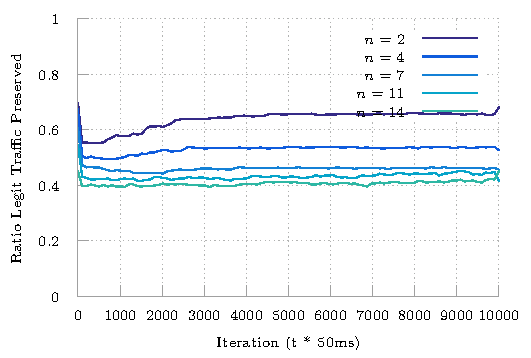
\includegraphics[width=\linewidth]{../plots/online-varyN-uneven}
	\caption{
		MARL pushback control system performance plotted over time, for various settings of $n$ hosts per learner.
		This plot shows that, from the perspective of benign hosts, service guarantees degrade as inference and applied actions become less granular.
		This generalises for all behavioural discriminators: even a perfect agent \emph{must} punish benign flows if they are grouped with malicious actors.
		\label{fig:marl-granularity}
	}
\end{figure}

\begin{figure}[ht]
	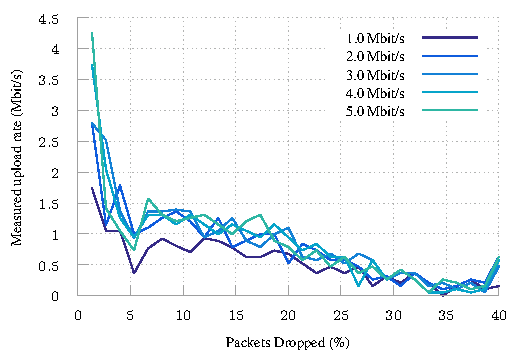
\includegraphics[width=\linewidth]{../plots/mplex}
	\caption{
		Average TCP upload rate of hosts targeting different bandwidths in \emph{mininet}, computed over 10 runs.
		As the rate of packet drop is linearly increased from \SIrange{0}{40}{\percent}, all flows begin to converge on an extremely low upload rate, regardless of the target bandwidth.
		This behaviour is to be expected, and is to the credit of the emulated environment---prior treatments have ignored such phenomena, which have strong implications on agent and network design.
		This confirms that packet drop does not affect benign TCP flows linearly, causing a higher rate reduction than what malicious flows will experience.
		\label{fig:mplex-tcp}
	}
\end{figure}

See above: a result.

?? Observations: training time lengthier by nature of emulated environment.
?? Risk of going for a simulation (i.e. numeric)? Always going to be interesting behaviour that is missed out on (in theory), at the cost of training time/limits of simulation speed

?? TCP perf characteristics under packet drop known by the Mathis equation \cite{DBLP:journals/ccr/MathisSMO97}:
\begin{equation}
\operatorname{BW} = \frac{\operatorname{MSS}}{\operatorname{RTT}} \frac{C}{\sqrt{p}},
\end{equation}
for the \emph{maximum segment size} (MSS), \emph{round trip time} (RTT), a choice of constant $C \approx{} \sqrt{3/2}$ dependent on system assumptions and the probability $p \in (0, 1]$ that a packet is lost.
The lower bound on $p$ is deliberately open, as packet drop acts as a control signal for the TCP send window size and is an expected part of normal operation.

\section{Related Work}

?? Other recent work in the prevention of DDoS? (i.e., non-RL).

%?? Abuses of RL 
Earnest, well-considered application of RL towards the challenge of intrusion detection/prevention has seen comparatively little examination.
Past work exhibits abuses of the paradigm as a glorified classifier for anomaly detection \cite{shamshirband2014anomaly} and DDoS prevention \cite{DBLP:conf/mates/ServinK08}.

?? Good Direct-control work \cite{DBLP:phd/ethos/Malialis14, DBLP:journals/eaai/MalialisK15}

?? Indirect-control applications: link to all the juicy stuff in e.g. HotNets, data-driven networking, the works. \cite{DBLP:conf/hotnets/ValadarskySST17, DBLP:conf/hotnets/MaoAMK16}.
The HMM stuff---learning when best to \emph{communicate} and share knowledge between explicit detector models \cite{DBLP:conf/paisi/XuSH07}.
The latter example's position is slightly weakened by its reliance on the discredited `DARPA99' dataset \cite{DARPA-IDD, DBLP:conf/cisda/TavallaeeBLG09, DBLP:conf/sp/SommerP10}, but the idea itself is well-treated and this acts as a driver for improvements in this direction.

\section{Conclusion}

It all ends here, Mr.\ Bond...

?? Please write me once everything else is in place.

?? Future Work? I.e., \emph{everything}: no one else is really looking at/interested in this specific kind of application of RL yet. \emph{Yet}.

?? Benefit of the more realistic emulation environ is that it is far closer in behaviour and architecture (i.e. viable) to a real SDN-enabled deployment, captures some dynamics which were otherwise hidden/lost by human ignorance. It also allows me to develop the system towards evolving traffic models where it is expected that RL should shine over and above standard ML techniques. Room to introduce/roll-in dynamic changepoint detection or adaptive exploration \cite{DBLP:conf/ki/Tokic10, DBLP:conf/ki/TokicP11, DBLP:conf/annpr/TokicP12}?

?? Overarching goal: works which respect the complexity of the network environment (rather than na\"{i}ve simulation, blind ML applications etc.) and choose well-considered pathways to solution. Call-to-action?

?? Security? I suspect that the very qualities that make inference difficult in IDS/IPS also increase the level of challenge an advanced threat must overcome.
System state which is dependent on many signals drawn from across a wide network, in concert with their burstiness and unpredictability, may have substantial effects on an attacker's capabilities.

\section*{Acknowledgements}
My thanks go to Dr.\ Dimitrios Pezaros for his supervision, guidance, and comments relating to the realisation of this work, and to Mircea Iordache and Richard Cziva for their comments and technical assistance.
Additional thanks \emph{would} go out to my anonymous reviewers, had I any of them.

\printbibliography

\end{document}